%%
%% This is file `sample-sigconf.tex',
%% generated with the docstrip utility.
%%
%% The original source files were:
%%
%% samples.dtx  (with options: `sigconf')
%% 
%% IMPORTANT NOTICE:
%% 
%% For the copyright see the source file.
%% 
%% Any modified versions of this file must be renamed
%% with new filenames distinct from sample-sigconf.tex.
%% 
%% For distribution of the original source see the terms
%% for copying and modification in the file samples.dtx.
%% 
%% This generated file may be distributed as long as the
%% original source files, as listed above, are part of the
%% same distribution. (The sources need not necessarily be
%% in the same archive or directory.)
%%
%% The first command in your LaTeX source must be the \documentclass command.
\documentclass[sigconf]{acmart}

\usepackage{latexsym}
\usepackage{makecell}
\usepackage[english]{babel}

%%
%% \BibTeX command to typeset BibTeX logo in the docs
\AtBeginDocument{%
  \providecommand\BibTeX{{%
    \normalfont B\kern-0.5em{\scshape i\kern-0.25em b}\kern-0.8em\TeX}}}


%% Rights management information.  This information is sent to you
%% when you complete the rights form.  These commands have SAMPLE
%% values in them; it is your responsibility as an author to replace
%% the commands and values with those provided to you when you
%% complete the rights form.
\copyrightyear{2021} 
\acmYear{2021} 
\setcopyright{acmcopyright}\acmConference[CIKM '21]{Proceedings of the 30th ACM
International Conference on Information and Knowledge Management}{November
1--5, 2021}{Virtual Event, QLD, Australia}
\acmBooktitle{Proceedings of the 30th ACM International Conference on Information
and Knowledge Management (CIKM '21), November 1--5, 2021, Virtual Event, QLD,
Australia}
\acmPrice{15.00}
\acmDOI{10.1145/3459637.3482097}
\acmISBN{978-1-4503-8446-9/21/11}

\newcommand{\secref}[1]{Section \ref{#1}}
\newcommand{\figref}[1]{Figure \ref{#1}}
\newcommand{\eqnref}[1]{Eq. (\ref{#1})}
\newcommand{\tabref}[1]{Table \ref{#1}}
\newcommand{\exref}[1]{Example \ref{#1}}
\newcommand{\cut}[1]{}
\newcommand{\KZ}[1]{\textcolor{blue}{Kenny: #1}}
\newcommand{\ZL}[1]{\textcolor{red}{Zhiling: #1}}

%%
%% Submission ID.
%% Use this when submitting an article to a sponsored event. You'll
%% receive a unique submission ID from the organizers
%% of the event, and this ID should be used as the parameter to this command.
%%\acmSubmissionID{123-A56-BU3}

%%
%% The majority of ACM publications use numbered citations and
%% references.  The command \citestyle{authoryear} switches to the
%% "author year" style.
%%
%% If you are preparing content for an event
%% sponsored by ACM SIGGRAPH, you must use the "author year" style of
%% citations and references.
%% Uncommenting
%% the next command will enable that style.
%%\citestyle{acmauthoryear}


%%
%% end of the preamble, start of the body of the document source.
\settopmatter{printacmref=true}
\begin{document}
\fancyhead{}% Remove all header contents

%%
%% The "title" command has an optional parameter,
%% allowing the author to define a "short title" to be used in page headers.
\title{Enriching Ontology with Temporal Commonsense for Low-Resource Audio Tagging}

%%
%% The "author" command and its associated commands are used to define
%% the authors and their affiliations.
%% Of note is the shared affiliation of the first two authors, and the
%% "authornote" and "authornotemark" commands
%% used to denote shared contribution to the research.

\author{Zhiling Zhang}
\affiliation{%
  \institution{Shanghai Jiao Tong University}}
\email{blmoistawinde@sjtu.edu.cn}
\orcid{0000-0002-8081-704X}

\author{Zelin Zhou}
\affiliation{%
  \institution{Shanghai Jiao Tong University}}
\email{ze-lin@sjtu.edu.cn}

\author{Haifeng Tang}
\affiliation{%
  \institution{CMB Credit Card Center}}
\email{thfeng@cmbchina.com}

\author{Guangwei Li*}
\affiliation{%
  \institution{Shanghai Jiao Tong University}}
\email{ligw20@sjtu.edu.cn}

\author{Mengyue Wu* $\dagger$}
\thanks{* authors are with MoE Key Lab of Artificial Intelligence and X-LANCE Lab}
\affiliation{%
  \institution{Shanghai Jiao Tong University}}
\email{mengyuewu@sjtu.edu.cn}
\thanks{$\dagger$ Corresponding author, supported by National Natural Science Foundation of China (No.61901265), 
Shanghai Pujiang Program (No.19PJ1406300), and Shanghai Municipal Science and Technology Major Project (2021SHZDZX0102).}

\author{Kenny Q. Zhu $\ddagger$}
\affiliation{%
  \institution{Shanghai Jiao Tong University}}
\email{kzhu@cs.sjtu.edu.cn}
\thanks{$\ddagger$ Corresponding author, and is partially supported by
SJTU-CMB Credit Card Center Joint Research Grant and SJTU Medical-Engineering
Cross Disciplinary Scheme.}
%%
%% By default, the full list of authors will be used in the page
%% headers. Often, this list is too long, and will overlap
%% other information printed in the page headers. This command allows
%% the author to define a more concise list
%% of authors' names for this purpose.
%\renewcommand{\shortauthors}{Zhang and Zhu}

%%
%% The abstract is a short summary of the work to be presented in the
%% article.
\begin{abstract}
  Audio tagging aims at predicting sound events occurred in a recording. Traditional models require enormous laborious annotations, otherwise performance degeneration will be the norm. Therefore, we investigate robust audio tagging models in low-resource scenarios with the enhancement of knowledge graphs. Besides existing ontological knowledge, we further propose a semi-automatic approach that can construct temporal knowledge graphs on diverse domain-specific label sets. Moreover, we leverage a variant of relation-aware graph neural network, D-GCN, to combine the strength of the two knowledge types. Experiments on AudioSet and SONYC urban sound tagging datasets suggest the effectiveness of the introduced temporal knowledge, and the advantage of the combined KGs with D-GCN over single knowledge source.
\end{abstract}

\begin{CCSXML}
<ccs2012>
    <concept>
        <concept_id>10010147.10010178.10010187</concept_id>
        <concept_desc>Computing methodologies~Knowledge representation and reasoning</concept_desc>
        <concept_significance>500</concept_significance>
        </concept>
  </ccs2012>
\end{CCSXML}

\ccsdesc[500]{Computing methodologies~Knowledge representation and reasoning}

%%
%% Keywords. The author(s) should pick words that accurately describe
%% the work being presented. Separate the keywords with commas.
\keywords{Audio Tagging, Low-Resource, Graph Neural Network, Knowledge Graph}

%%
%% This command processes the author and affiliation and title
%% information and builds the first part of the formatted document.
\maketitle

\section{Introduction}

Protein$-$protein interactions (PPIs) are of central importance for the majority of biological functions, such as signal transduction, metabolic pathways, molecular dynamics, and protein networks\cite{Hoffmann.Krallinger.ea:2005}, for they serve as the most fundamental building blocks of the entire interacademic systems of any organisms. Collecting data on pairwise interaction relationships is essential for multiple purpose, including identification of modules with certain functionality\cite{Spirin.Mirny.03}, mapping diseases to dominated genes\cite{Ideker.Sharan.08}, and after all, understanding wholistic metabolic/genetic networks from a system biology perspective.

A lot of databases have been built to store protein and genetic interactions from major model organism species and are available in various standardized formats, such as MINT\cite{Zanzoni.Montecchi-Palazzi.ea:2002}, BIND\cite{Bader.ea:2003}, BIOGRID\cite{DBLP:journals/nar/StarkBRBBT06}, etc. Among those mainstream databases, the data largely rely on voluntary reports by scientists or researchers, besides, comprehensive curation efforts become indispensable for the sake of accuracy. However, the amount of biology-related literatures with respect to protein interactions grows explosively and thus make it either impossible or impractical to manually detect PPI information anymore.

Considering huge amount of PPI information with great wealth hidden in published papers, in recent years, numerous mining techniques have been proposed that aim to extract PPI information automatically from free text, especially machine learning, information retrieval, and natural language processing\cite{DBLP:journals/bib/WinnenburgWPDS08}.These approaches can be roughly categorized into three classes: co$-$occurrence, rule$-$based, and machine learning. 

Co$-$occurrence is the approach with most simplicity and naivete. Just as its name implies, this method intends to find out pairs of proteins that co-occur in the same context. The scope of "same context" ranges from phrase, sentence, paragraph to whole abstract, even document. The underlying assumption is that whenever two proteins are mentioned together by authors, chances are high that there is some kind of relationship between them. However, however, in-context closeness even semantic relation does not necessarily represent actual biological interaction. As a consequence, a large fraction of candidate pairs are mismatched inevitably, causing a high recall but low precision.

The second approach is rule-based extraction, in other words, pattern matching. There are many types of rules, most of them concern natural language processing (NLP). One way is to specify hand-crafted regular expressions before hand, which mostly lean on language usage preference. Besides, by using full or partial (shallow) parsing strategies, more information would be acquired, such as part-of-speech taggers, local dependencies between syntactic components, context-free grammar\cite{DBLP:journals/bioinformatics/TemkinG03}, and full sentence structure. Compared to co$-$occurrence, rule-based approach enjoy better precision but much lower recall. In addition, since the rules are usually derived from training data, that is to say, the improper choice of training data would be significantly lethal, therefore quality of extraction is invariably instable and may not applicable to other data.

The third and most commonly used approach use machine learning techniques, in this case, the task to extract protein$-$protein interactions turns out to be a binary classification problem. Each protein pairs are represented along with a set of features, which is associated with their context, then a well$-$defined classifier gives the answer whether the candidate protein pairs is classified to be qualified PPI. (TO BE FURTHER FILLED!!!)

In this paper, we introduce a general bootstrapping framework for Protein$-$protein interaction extraction from natural text.Our method differs from most of the previous works in three aspects:

(1)The extraction process is driven by only tiny fraction of training data, which are regarded as seed data. In each round, it would derive reliable patterns automatically from seed data, then extract more positive PPI pairs consequently, what's more, the seed data would be augmented by the newly extracted results with high confidence.

(2)multiple graph kernel. 

(3)various evaluation.




\section{Approach}
%We first present our methods for testing short circuits in
%models, then modify some of these methods to create
%training data to reverse the short circuit problem
%and enhance the robustness of the models.
% 
%\subsection{Proxy Test for Short Circuit}
%We propose two types of approaches that can be used as proxy test for short circuits.
%One is through inspecting attention maps in
%the models under a white-box setting.
%The other is to generate new test cases by applying different operations on correct choices under a black-box setting.
%
%
%\subsubsection*{White-box Attention Weights~(AW)}
%One intuitive way to detect if an attention-based model is 
%exploiting short circuits is to visualize its attention map. 
%Given a well-trained model and a correctly answered MCQ  in the 
%form of \textit{[CLS] premise [SEP] choice [SEP]}, 
%where \textit{[CLS]} and \textit{[SEP]} are model-dependent 
%delimiters and \textit{choice} refers to the correct choice, 
%we first tokenize the input, feed the token sequence into the model, 
%and extract the attention map of all attention heads from the 
%last encoder layer.
%
%The attention maps are visualized through off-the-shelf tool~\cite{vig-2019-multiscale}
%into user-friendly demo as shown in \figref{fig:att-goodex}. 
%Human annotators are then asked to determine whether there exists 
%strong attention connections from the correct choice to the premise. 
%We consider the MCQ is solved without short-circuiting only if 
%over half of the annotators label it as having strong attention 
%connections. 
%
%Though accurate, such manual annotation is cost-prohibitive to be 
%scaled to larger tests. To remedy this issue, we propose 
%a rule-based procedure to automatically detect the short circuit 
%behavior of a model on MCQ. Specifically, we aggregate the 
%attention maps into one individual map by max-pooling over all 
%attention heads. Then we check if there exists at least one 
%attention score between token in the choice and token in the premise 
%higher than threshold $t_1$ or at least two higher than threshold 
%$t_2$, excluding special tokens like comma and period. 
%We consider that the model not short-circuiting on this MCQ if 
%neither of the two conditions is met. In practice, the 
%threshold $t_1$ and $t_2$ are tuned so as to maximally simulate 
%human annotation. The pseudo-code is shown in Algorithm \ref{AW}.
%
In this section, we first present our methods for testing short circuits in models, and then modify some of these methods to create training data to address the short circuit problem and enhance model robustness.

\subsection{Proxy Test for Short Circuit}
Since no existing method can definitively prove if a model is short-circuiting on a question, we propose two types of approaches that serve as proxy tests for short circuits. These approaches reveal the effects of model short-circuiting, though they can't directly prove the short-circuit itself, similar to dark matter. One approach involves inspecting attention maps in models under a white-box setting, while the other generates new test cases by applying different operations on correct choices under a black-box setting.

\subsubsection*{White-box Attention Weights~(AW)}

One intuitive way to detect if an attention-based model is exploiting short circuits is to visualize its attention map. Given a well-trained model and a correctly answered MCQ in the form of \textit{[CLS] premise [SEP] choice [SEP]}, where \textit{[CLS]} and \textit{[SEP]} are model-dependent delimiters and \textit{choice} refers to the correct choice, we first tokenize the input, feed the token sequence into the model, and extract the attention map of all attention heads from the last encoder layer.

The attention maps are visualized through an off-the-shelf tool~\cite{vig-2019-multiscale} into a user-friendly demo, as shown in \figref{fig:att-goodex}. Human annotators are then asked to determine whether there exists strong attention connections from the correct choice to the premise. We consider the MCQ to be solved without short-circuiting only if over half of the annotators label it as having strong attention connections.

Although accurate, such manual annotation is cost-prohibitive to be scaled to larger tests. To remedy this issue, we propose a rule-based procedure to automatically detect the short circuit behavior of a model on MCQ. Specifically, we aggregate the attention maps into one individual map by max-pooling over all attention heads. Then we check if there exists at least one attention score between a token in the choice and a token in the premise higher than threshold $t_1$, or at least two higher than threshold $t_2$, excluding special tokens like comma and period. We consider the model to not be short-circuiting on this MCQ if neither of the two conditions is met. In practice, the thresholds $t_1$ and $t_2$ are tuned to maximally simulate human annotation. The pseudo-code is shown in Algorithm \ref{AW}.


\begin{algorithm}
\small
	\caption{Attention Weight Thresholding}
	\label{AW}
\hspace*{0.02in} {\bf Input:} 
premise $P$, correct choice $C$, model $M$,  threshold $t_1$ and $t_2$. \\
\hspace*{0.02in} {\bf Output:}
binary 0/1 label $L$.
	\begin{algorithmic}[1]
		\State initialize counters $c_1$ and $c_2$ to 0.
		\State tokenize the formatted input as sequence of tokens $S$.
		\State feed $S$ into $M$ and extract the last layer's attention maps $Attn_{all}$.
		\State aggregate $Attn_{all}$ into $Attn_{max}$ by max-pooling over all attention heads.
		\For{$w_1$ in $C$}
		\For{$w_2$ in $P$}
		\If{$Attn_{max}(w_1, w_2)> t_1$}
				$c_1$ += 1
		\EndIf
		\If{$Attn_{max}(w_1, w_2) > t_2$}
				$c_2$ += 1
		\EndIf
		\EndFor
		\EndFor
		\State output 1 if $c_1>0$ or $c_2\geq 2$ and 0 otherwise.
	\end{algorithmic}
\end{algorithm}

\subsubsection*{Black-box Choice Operator}
\label{sec:proxy}
While attention-based testing methods can detect short circuits within the encoder directly, they don't directly detect short circuits in the end-to-end MCQ model, which also includes a linear layer above the attention-based pretrained language model. Additionally, these methods are limited to a family of models with inherent attention mechanisms.

A more desirable approach is an automatic end-to-end black-box test that is model-independent. In black-box testing, if a model correctly answers an MCQ, we slightly modify the MCQ by applying a certain``operation'' on the original correct choice to produce another wrong choice. The newly generated MCQ must share the same correct choice as the original question. By observing the model's response to the second MCQ, we can infer whether the model short-circuits on the original MCQ.If the model still selects the correct choice, then we consider it to have passed the test and not short-circuited on the original MCQ. The challenge now is how to construct the new wrong choice by implementing the operation in various ways.

In this paper, we consider the operations listed in \tabref{table:proxyop}. Some of the operations were mentioned in previous literature, while others are proposed here (marked with *).
The first line in each cell describes the operation, and the next two lines provide an example of constructing a false choice from a choice in the original question. An operation may either preserve (p) the truth value (\crosssymbol $\rightarrow$ \crosssymbol) or change (c) the truth value of the choice (\checksymbol $\rightarrow$ \crosssymbol).

\begin{table}[th]
        \centering
        \scriptsize
        \begin{tabular}{l|l}
                \toprule
                \textbf{Oper.} &\textbf{Description and Example}\\
                \hline
                \multirow{3}{*}{Neg+} & Add negation (c) \\
                & \textit{They called the police to come to my house. \checksymbol} \\
                & \textit{They {\color{olive}{didn't}}  called the police to come to my house. \crosssymbol} \\
                \hline
                \multirow{3}{*}{Neg-} &Remove negation (c) \\
                & \textit{Ben {\color{olive} never} starts working out. \checksymbol} \\
                & \textit{Ben starts working out. \crosssymbol}\\
                \hline

                \multirow{3}{*}{NER} &Randomly replace person names (c)\\
                 & \textit{A big wave knocked {\color{olive} Mary} down . \checksymbol} \\
                & \textit{A big wave knocked {\color{olive} Kia} down . \crosssymbol} \\
                \hline
                \multirow{3}{*}{PR*} & Switch pronoun by gender or quantity (c)\\
        &\textit{{\color{olive} She} had a great time .\checksymbol} \\
        &\textit{{\color{olive} He} had a great time . \crosssymbol} \\
                \hline
                \multirow{3}{*}{PI*} &Instantiate pronoun by randome person (c) \\
        &\textit{{\color{olive} They} gave Tom a new latte with less ice . \checksymbol}\\
        &\textit{{\color{olive} Nathanael} gave Tom a new latte with less ice . \crosssymbol}\\
                \bottomrule
%               \hline
                \multirow{3}{*}{Adv} &Add adverbs for emphasis (c) \\
                &\textit{The ocean was a calm as a bathtub .\crosssymbol} \\
                &\textit{{\color{olive} In fact} the ocean was a calm as a bathtub .\crosssymbol} \\
                \hline
               \multirow{3}{*}{CO*} & Crossover: Swap the true choices between two questions (p)\\ 
	&\textit{\color{olive}Josh got sick . \checksymbol} \\
	&\textit{\color{olive}{She had a great time .\crosssymbol}}  \\
\hline
                \multirow{3}{*}{Syn} &Replace adj/adv with synonym (p) \\
                &\textit{Dawn felt {\color{olive} happy} about getting away with it . \crosssymbol} \\
                &\textit{Dawn felt {\color{olive} glad} about getting away with it . \crosssymbol} \\

		\bottomrule
               \multirow{3}{*}{MT*} & Mutate: Swap two consecutive words (c) \\
		& \textit{Deb said yes {\color{olive} to} {\color{olive} Tim} 's marriage proposal. \crosssymbol} \\
		& \textit{Deb said yes {\color{olive} Tim} {\color{olive} to} 's marriage proposal .\crosssymbol} \\
               \hline
\multirow{3}{*}{Voice} &Swap subject and object (c) \\
        & \textit{{\color{olive}{Kara}} asked {\color{olive}{the neighbors}}  not to litter in their yard . \checksymbol} \\
        &\textit{{\color{olive}{the neighbors}} asked  {\color{olive}{Kara}}  not to litter in their yard . \crosssymbol}\\
                \bottomrule
        \end{tabular}
        \caption{A number of operations considered for proxy testing. 
First line in each cell describes the operation, the next two lines
give an example of how to construct a false choice from a choice of
the original question. An operation may either 
preserve (p) the truth value (\checksymbol $\rightarrow$ \checksymbol, \crosssymbol $\rightarrow$ \crosssymbol) or change (c) the truth value of
the choice (\checksymbol $\rightarrow$ \crosssymbol).  }
        \label{table:proxyop}
\end{table}

Inspired by boundary testing in software engineering, we can classify these operations into three equivalent classes (three vertical sections in \tabref{table:proxyop}), depending on the nature of the \textit{false} choice constructed:
\begin{enumerate}
\item The syntax and semantics are correct, and the \textit{false} choice appears similar to the \textit{true} choice.
\item The syntax and semantics are correct, and the \textit{false} choice appears distinct from the \textit{true} choice.
\item Either syntax or semantics is incorrect.
\end{enumerate}

The last class is not suitable for testing short circuits because the model may answer the proxy question correctly by eliminating the false choice due to errors in it, not by considering the premise.

We focus on perturbations on negation~\cite{checklist2020acl}, NER~\cite{checklist2020acl}, and pronouns in the first class and adverbial~\cite{wsp2020acl}, crossover, and synonym~\cite{checklist2020acl,wsp2020acl} in the second class.

While most of the operations are self-explanatory, the \textit{crossover} operation is unique and deserves special attention. Inspired by molecular biology, for each MCQ in the dataset that the model answers correctly, we substitute the original false choice with the true choice from another randomly sampled MCQ. The substituted choice remains false in the proxy question. The operation can be visually explained in \figref{fig:cross}.

\begin{figure}[th]
\centering
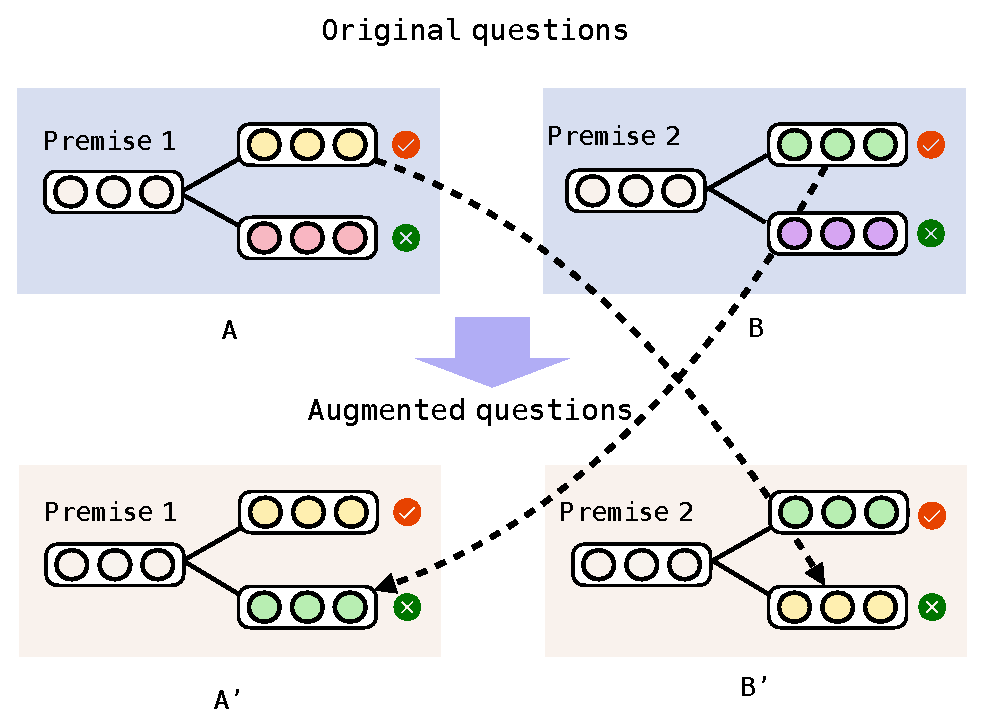
\includegraphics[width=\columnwidth]{figure/cross.eps}
\caption{The Crossover Operation: the true choice of both questions
are used to replace the false choices of these questions to create
two new proxy questions.}
\label{fig:cross}
\end{figure}

Compared to all other operations in classes 1 and 2, the crossover provides a proxy question that is most different from the original one but easier from a human perspective. This is because the two choices may be quite unrelated. If the model does not handle it correctly, it may be more indicative of a short circuit. As a result, the crossover is potentially a better short circuit test than others.

Another advantage of the crossover operation is that we can generate multiple false choices for an original question at a low cost, allowing us to test each original question more thoroughly. In contrast, most other operations cannot produce an adequate number of different variants of the original choice.

In summary, the proposed black-box choice operator provides a more generalizable and model-independent method for detecting short circuits in MCQ models. By applying various operations to create proxy questions, we can assess the model's performance and robustness more accurately, contributing to the development of better and more reliable models in the future.

\subsection{Improving Model Robustness by Data Augmentation}

If a model is shown to short-circuit by the proxy tests, its performance may decline, especially when applied to out-of-domain test data. To make models more robust, one natural thought is to generate more data to encourage models to focus on the relation between the premise and choices. While the operations used to generate proxy tests can also be utilized for data augmentation, not all of them are scalable or able to generate enough data for training.

The two operations that can generate a substantial amount of data are crossover and mutation. These operations can be applied to the training data to enhance the model's robustness.

\subsubsection*{Crossover for Data Augmentation}

Crossover is a good option for data augmentation because the two choices were originally true answers in their respective questions and presumably carry spurious features if the model was short-circuiting. By incorporating crossover into the training data, the model is forced to consider the premise in order to determine which choice is better.

\subsubsection*{Mutation for Data Augmentation}

Mutation has two flavors: (1) swap the words only in the true choice; (2) swap the words both in the true and the false choice. Compared to crossover, mutation has the potential to be more effective at improving model robustness. It not only forces the model to look into the premise due to its two very similar choices (same set of tokens), but also makes the model more sensitive to fine differences in word orders and enhances the model's prior grammatical knowledge.

\subsubsection*{Differentiating between Proxy Test and Data Augmentation}

It is essential to differentiate between the use of crossover and mutation operations in proxy tests and data augmentation. In proxy tests, these operations are used to modify the test data to assess the model's short-circuiting behavior. In contrast, when applied for data augmentation, the same operations work on the training data to enhance the model's robustness and generalization capabilities.

In conclusion, data augmentation through crossover and mutation operations can contribute to improving model robustness by encouraging models to focus on the relationship between the premise and choices. By incorporating these operations into the training data, models are forced to consider the premise and become more sensitive to the fine differences in word orders, leading to better performance and reliability in real-world applications.

\section{Experiments}
\label{sec:experiments}

% \subsection{Datasets and Metrics}

We experiment our methods on datasets with corresponding ontologies to verify the effectiveness of either ontological or temporal knowledge alone, and their combination.

\textit{AudioSet} is a large-scale multi-label audio tagging dataset collected from Youtube videos with the annotations of 527 categories out of the 632 tags defined in the ontology. Most recordings are processed into 10 seconds single-channel 16kHz, 16-bit wave format. Due to the changes of videos, it is not possible to recover the whole dataset. We downloaded 19,400 (87.5\%), 1,851,420 (90.7\%), and 17,756 (87.2\%) recordings for the balanced train, full train, and evaluation set, respectively. To simulate the low-resource scenario, we randomly sample 1\% of the unbalanced set as the training set, which has 18,514 samples, where 134 classes have no more than 5 samples, and 10 classes have no training sample. We also sample 5\% and 10\% sets for comparison. We use the commonly used mAP, mAUC as the evaluation metrics. 
\textit{SONYC} is the multi-label Urban Sound Tagging dataset used in DCASE 2019 Task5 (D19T5). It contains 2,351 train recordings and 443 validate recordings, which can be considered relatively low-resource. All recordings are 10 seconds single-channel 44.1kHz, 16-bit wave format. We use the official metrics, micro AUPRC and macro AUPRC.

\subsection{Experimental Setup}

\paragraph{Audio Features} For SONYC, we adopt a similar setting as \citep{kong2019cross}, all audios are re-sampled to 32 kHz and 64-Mel-bin log-Mel spectrograms are used to to represent the audios. The window size is 1024 samples, the hop size of 500 samples, and cut-off frequencies of 50 Hz to 14 kHz. 
For AudioSet, our setting is similar to \citep{kong2020panns}, all audios are re-sampled to 16 kHz and represented as 64-Mel-bin log-Mel spectrograms. The window size is 512 samples, the hop size of 160 samples, and cut-off frequencies of 50 Hz to 8 kHz.

\paragraph{Models and Baselines} We adopt standard CNN models as our baseline, that is, the CNN9 model use in \citep{kong2019cross} for SONYC and the CNN14 (16kHz) in \citep{kong2020panns} for AudioSet. We also introduce the SOTA method AT-GCN \citep{wang2020modeling} as baseline, which is based on co-occurrence graph mined from the whole AudioSet annotation, and uses tuned, dataset-specific hyperparameter for edge thresholding and smoothing. It is thus not directly applicable to SONYC. Our models include GCN(ASER), GCN(AudioSet), GCN(ASER+AudioSet), which refers to single GCN with temporal knowledge, AudioSet ontology, and their combination. D-GCN denotes double-GCN with 2 types of knowledge. We replace AudioSet with SONYC's ontology (OT) for experiments on SONYC dataset. We use batch size of 32 for all models and the learning rate is 1e-3 for all models except D-GCN using 3e-4.

\subsection{Results}

\subsubsection{AudioSet}


\begin{table}[tbp]
  \setlength{\belowcaptionskip}{-0.cm}
  \centering
  \small
  \begin{tabular}{lcccc}
      \hline
      {} & \multicolumn{2}{c}{Balance} & \multicolumn{2}{c}{Unbalance (100\%)} \\
      \cline{2-3}\cline{4-5} 
      Methods & mAP & mAUC & mAP & mAUC \\
      \hline
      CNN14 & 0.2441 & 0.8930 & 0.4090 & 0.9669 \\
      \hline
      AT-GCN & 0.2510 & 0.9278 & 0.4095 & 0.9664 \\
      GCN(ASER) & 0.2500 & 0.9283 & 0.3994 & 0.9660 \\
      GCN(AudioSet) & 0.2543 & \textbf{0.9420} & 0.4063 & 0.9665 \\
      GCN(ASER+AudioSet) & 0.2490 & 0.9277 & 0.3999 & \textbf{0.9690} \\
      D-GCN & \textbf{0.2554} & 0.9377 & \textbf{0.4109} & 0.9648 \\
      \hline
  \end{tabular}
  \caption{\label{tab:bal-unbal} Results on AudioSet evaluation set with models trained on balanced and unbalanced set.}
\end{table}

\begin{table}[tbp]
  \setlength{\belowcaptionskip}{-0.cm}
  \centering
  \small

  \begin{tabular}{lccc}
      \hline
      Methods &     1\% &     5\% &    10\% \\
      \hline
      CNN14                 & 0.1118 & 0.2343 & 0.2770 \\
      \hline
      AT-GCN                & 0.1243 & 0.2331 & 0.2785 \\
      GCN(ASER)             & 0.1252 & 0.2269 & 0.2735 \\
      GCN(AudioSet)         & 0.1280 & 0.2336 & 0.2747 \\
      GCN(AudioSet+ASER)    & 0.1214 & 0.2283 & 0.2741 \\
      D-GCN  & \textbf{0.1283} & \textbf{0.2387} & \textbf{0.2799} \\
      \hline
      D-GCN rel. improvement & 14.73\% & 1.88\% & 1.05\% \\
      \hline
  \end{tabular}   
  \caption{\label{tab:low-resource-map} mAP for each model trained on different portion of the unbalanced set, and the relative improvement(\%) of D-GCN over CNN14 backbone.}
  \vspace{-4mm}
\end{table}


\tabref{tab:bal-unbal} shows the performance of models trained on the official balanced and unbalanced set, while \tabref{tab:low-resource-map} shows the results on sampled subsets. We can see that all GCN-based models significantly outperform the baseline CNN14 on balanced and low-resource (1\%) set, suggesting the usefulness of the knowledge sources including the newly proposed temporal knowledge in low-resource scenarios. As the size of training data grows, the advantage of GCN models ceases to exist, expect for AT-GCN, possibly due to its knowledge of the co-occurrences on the whole training set, which matches more with the larger training data. D-GCN performs consistently better than single GCN with one KG or the simple addition of both KGs, showing the effectiveness of the separate relation modeling, and it also outperforms CNN14 by mAP in all settings despite the diminishing gain.

To study the reason for the effectiveness of GCN models in low-resource scenario (1\% set) and their degeneration in large-data settings, we divide the classes into groups according to the numbers of training samples, and calculate D-GCN's improvement over baseline on these groups. From Figure \ref{fig:delta_map_auc}, we can see that D-GCN can benefit classes with extremely few samples ([0, 5]), and the gain is the highest on classes with moderate number of samples, but not on the most prevalent classes. We may conclude that the prior knowledge in KG can effectively help the model learn the dependency between labels especially for the few-shot ones. However, as we have more resources, the large backbone model may be capable of learning such relations without KG, which explains why the advantage of GCN-based models would shrink.   

\begin{figure}[htbp]
\setlength{\abovecaptionskip}{0.cm}
\setlength{\belowcaptionskip}{-0.5cm}
\centering
\includegraphics[width=0.9\linewidth]{figures/1p_delta_map_auc.pdf}
\caption{Absolute improvement of D-GCN over CNN14 on classes with different number 
of training samples.}
\label{fig:delta_map_auc}
\end{figure}

\subsubsection{SONYC}

\begin{table}[tbp]
  \setlength{\belowcaptionskip}{-0.cm}
    \centering
    \small
    \begin{tabular}{lcccc}
        \hline
        {} & \multicolumn{2}{c}{Fine-level} & \multicolumn{2}{c}{Coarse-level} \\
        \cline{2-3}\cline{4-5} 
        Methods & Mi AUPRC & Ma AUPRC & Mi AUPRC & Ma AUPRC \\
        \hline
        CNN9 & 0.675 & 0.493 & 0.808 & 0.580 \\
        GCN(ASER) & 0.703 & 0.459 & 0.822 & 0.548 \\
        GCN(OT) & 0.680 & 0.494 & 0.821 & 0.596 \\
        GCN(ASER+OT) & 0.706 & 0.492 & \textbf{0.823} & 0.616 \\
        D-GCN & \textbf{0.709} & \textbf{0.516} & 0.820 & \textbf{0.647} \\
        \hline
    \end{tabular}
    \caption{\label{tab:SONYC} Results on SONYC validate set, OT: SONYC ontology, Mi: Micro, Ma: Macro.}
    \vspace{-4mm}
  \end{table}

The results on the SONYC dataset is shown in Table \ref{tab:SONYC}. Similar to AudioSet (1\%), all GCN models significantly outperform baseline by the main metric Micro AUPRC. The temporal knowledge of ASER seems to be more useful here compared to ontology, as the ontology for SONYC is more sparse, and the labels for each level are predicted separately, so that they don't co-occur. D-GCN again gives consistently best or competitive performance on both level, suggesting the generalizability of this method on effectively combining the strength of two knowledge types.

\section{Conclusion}
We implement a novel sequence-based dependency parsing
framework which takes advantage of high order features 
in parsing history. 
%We can also adapt beam search to this framework so as to
%relax the strictly greedy nature. Vine pruning\cite{rush2012vine} could
%be incorporated to speed up the parsing.
More importantly, we discovered that the parsing accuracy is very sensitive to
the quality of parsing sequence. Future work can be focused on
developing better sequence predictors that outperform Malt action classifier.
Furthermore, we use two sets of features for sequence predictor and
head mapper right now. A unified set of features between these two components
are worth exploring.
%Besides, better sequence predicting method and unified feature
%representation of two components are worth exploring.
%
%Though we currently get a not bad result,
%the sequence predictor still needs more exploration.
%According to our experiment, slightly changes
%on the sequence can lead to a fatal decline on accuracy. Ensuring the match degree of training sequence and testing
%sequence demands a high quality of sequence predictor.
%
%Further, the features in our current implementation are not expanded and well tuned yet  and we are free to define high order features to make use of parsing history. Our framework is flexible to merge other technics to enhance the performance. Introducing beam could make up for our greedy decoder and improve our accuracy. Vine pruning\cite{rush2012vine} could speed up parsing process. Besides, better sequence predicting method and unified feature representation of two components are worth exploring.



%\begin{acks}
%TODO
%\end{acks}


%%
%% The next two lines define the bibliography style to be used, and
%% the bibliography file.
\bibliographystyle{ACM-Reference-Format}
\bibliography{cikm}

%%
%% If your work has an appendix, this is the place to put it.
\appendix

% \begin{table*}[th]
    \centering
    \tiny
    \resizebox{\linewidth}{!}{
        \begin{tabular}{cccccccc}
        \hline
        \textbf{Case} & \textbf{Character} & \textbf{Initial} & \textbf{Final} & \textbf{Rule} & \textbf{Initial IPA} \\
        \hline
        direct                      & \begin{CJK*}{UTF8}{gbsn}波\end{CJK*} &  \begin{CJK*}{UTF8}{gbsn}帮\end{CJK*} & \begin{CJK*}{UTF8}{gbsn}戈\end{CJK*} & \begin{CJK*}{UTF8}{gbsn}帮\end{CJK*}=[p] and \begin{CJK*}{UTF8}{gbsn}戈\end{CJK*}=[\textipa{uA}] & [p] \\
        \multirow{2}{*}{rule-based} 
        & \begin{CJK*}{UTF8}{gbsn}砩\end{CJK*} & \begin{CJK*}{UTF8}{gbsn}帮\end{CJK*} & \begin{CJK*}{UTF8}{gbsn}废\end{CJK*} & \multirow{2}{*}{if(initial=\begin{CJK*}{UTF8}{gbsn}帮\end{CJK*} and final=\begin{CJK*}{UTF8}{gbsn}废\end{CJK*}) then [f] else [p]} & [f] \\
        & \begin{CJK*}{UTF8}{gbsn}碑\end{CJK*} & \begin{CJK*}{UTF8}{gbsn}帮\end{CJK*} & \begin{CJK*}{UTF8}{gbsn}支\end{CJK*} &  & [p] \\
        arbitrary                   & \begin{CJK*}{UTF8}{gbsn}方\end{CJK*} & \begin{CJK*}{UTF8}{gbsn}帮\end{CJK*} & \begin{CJK*}{UTF8}{gbsn}阳\end{CJK*} & - & [f] \\
        \hline
        converted                   & \begin{CJK*}{UTF8}{gbsn}比\end{CJK*} & \begin{CJK*}{UTF8}{gbsn}帮\end{CJK*} & \begin{CJK*}{UTF8}{gbsn}旨\end{CJK*} & - & [p]\\
        \hline				
        \end{tabular}
        }
    \caption{Five different examples of reconstruction.}
    \label{tab:reconstruction}
\end{table*}
\section{Different Cases of Reconstruction}
\label{app:reconstruction}
\tabref{tab:reconstruction} presents five examples in four different cases constructing our ancient Chinese pronunciation dataset for each category. For an identical initial category, different rules applied can lead to different reconstruction result for initial IPA.

\section{Embedding for Medial Feature, Nucleus Feature, and Coda Feature}
\label{app:embedding}
This appendix supplements the embedding employed for the medial, nucleus, and coda features in GTenhanced Transformer, as shown in \figref{fig:embedding2}.

\begin{figure*}[th]
    \centering
    \includegraphics[width=0.4\textwidth]{images/embedding_layer2.png}
    \caption{Embedding for medial feature, nucleus feature, and coda feature.}
    \label{fig:embedding2}
\end{figure*}



\end{document}
\endinput
%%
%% End of file `sample-sigconf.tex'.
